%\section{Systemmodelle}
\newpage
\subsection{Anwendungsfalldiagramm}
Das System ist in die Benutzergruppe HIWI, Betreuer und Admin unterteilt. Folgendes Use-Case-Diagramm beschreibt die Interaktionsmöglichkeiten der einzelnen Benutzergruppe mit dem Server:
\begin{itemize}
	\item Mit dem Accounts Verwalten kann der Admin neuen Benutzer anlegen, Account abändern, Rechte vergeben oder löschen.
	\item Mit Komponente Login können Benutzer sich anmelden bzw. abmelden.
	\item Eine HiWi kann neue Zeiterfassung starten. Nachträgliche Erfassung, Bearbeitung oder Korrektur ist möglich. Er darf seine eigene erfasste Zeiten und Stundenzettel ansehen. Er kann Warnungen und Erinnerungen lesen. Er druckt sein Stundenzettel aus, unterschreibt und gibt es bei seinem Betreuer ab.
	\item Ein Betreuer darf die Erfasste Zeiten, Stundenzettel, und Nachrichten von allen seinen zugewiesenen HiWis ansehen. Er kontrolliert Stundenzettel von seinen HiWis und gibt die Status weiter an den Admin.
	\item Der Admin dürfen alles ansehen. Außderdem sammelt er noch alle Stundenzettel ein.
\end{itemize}\\


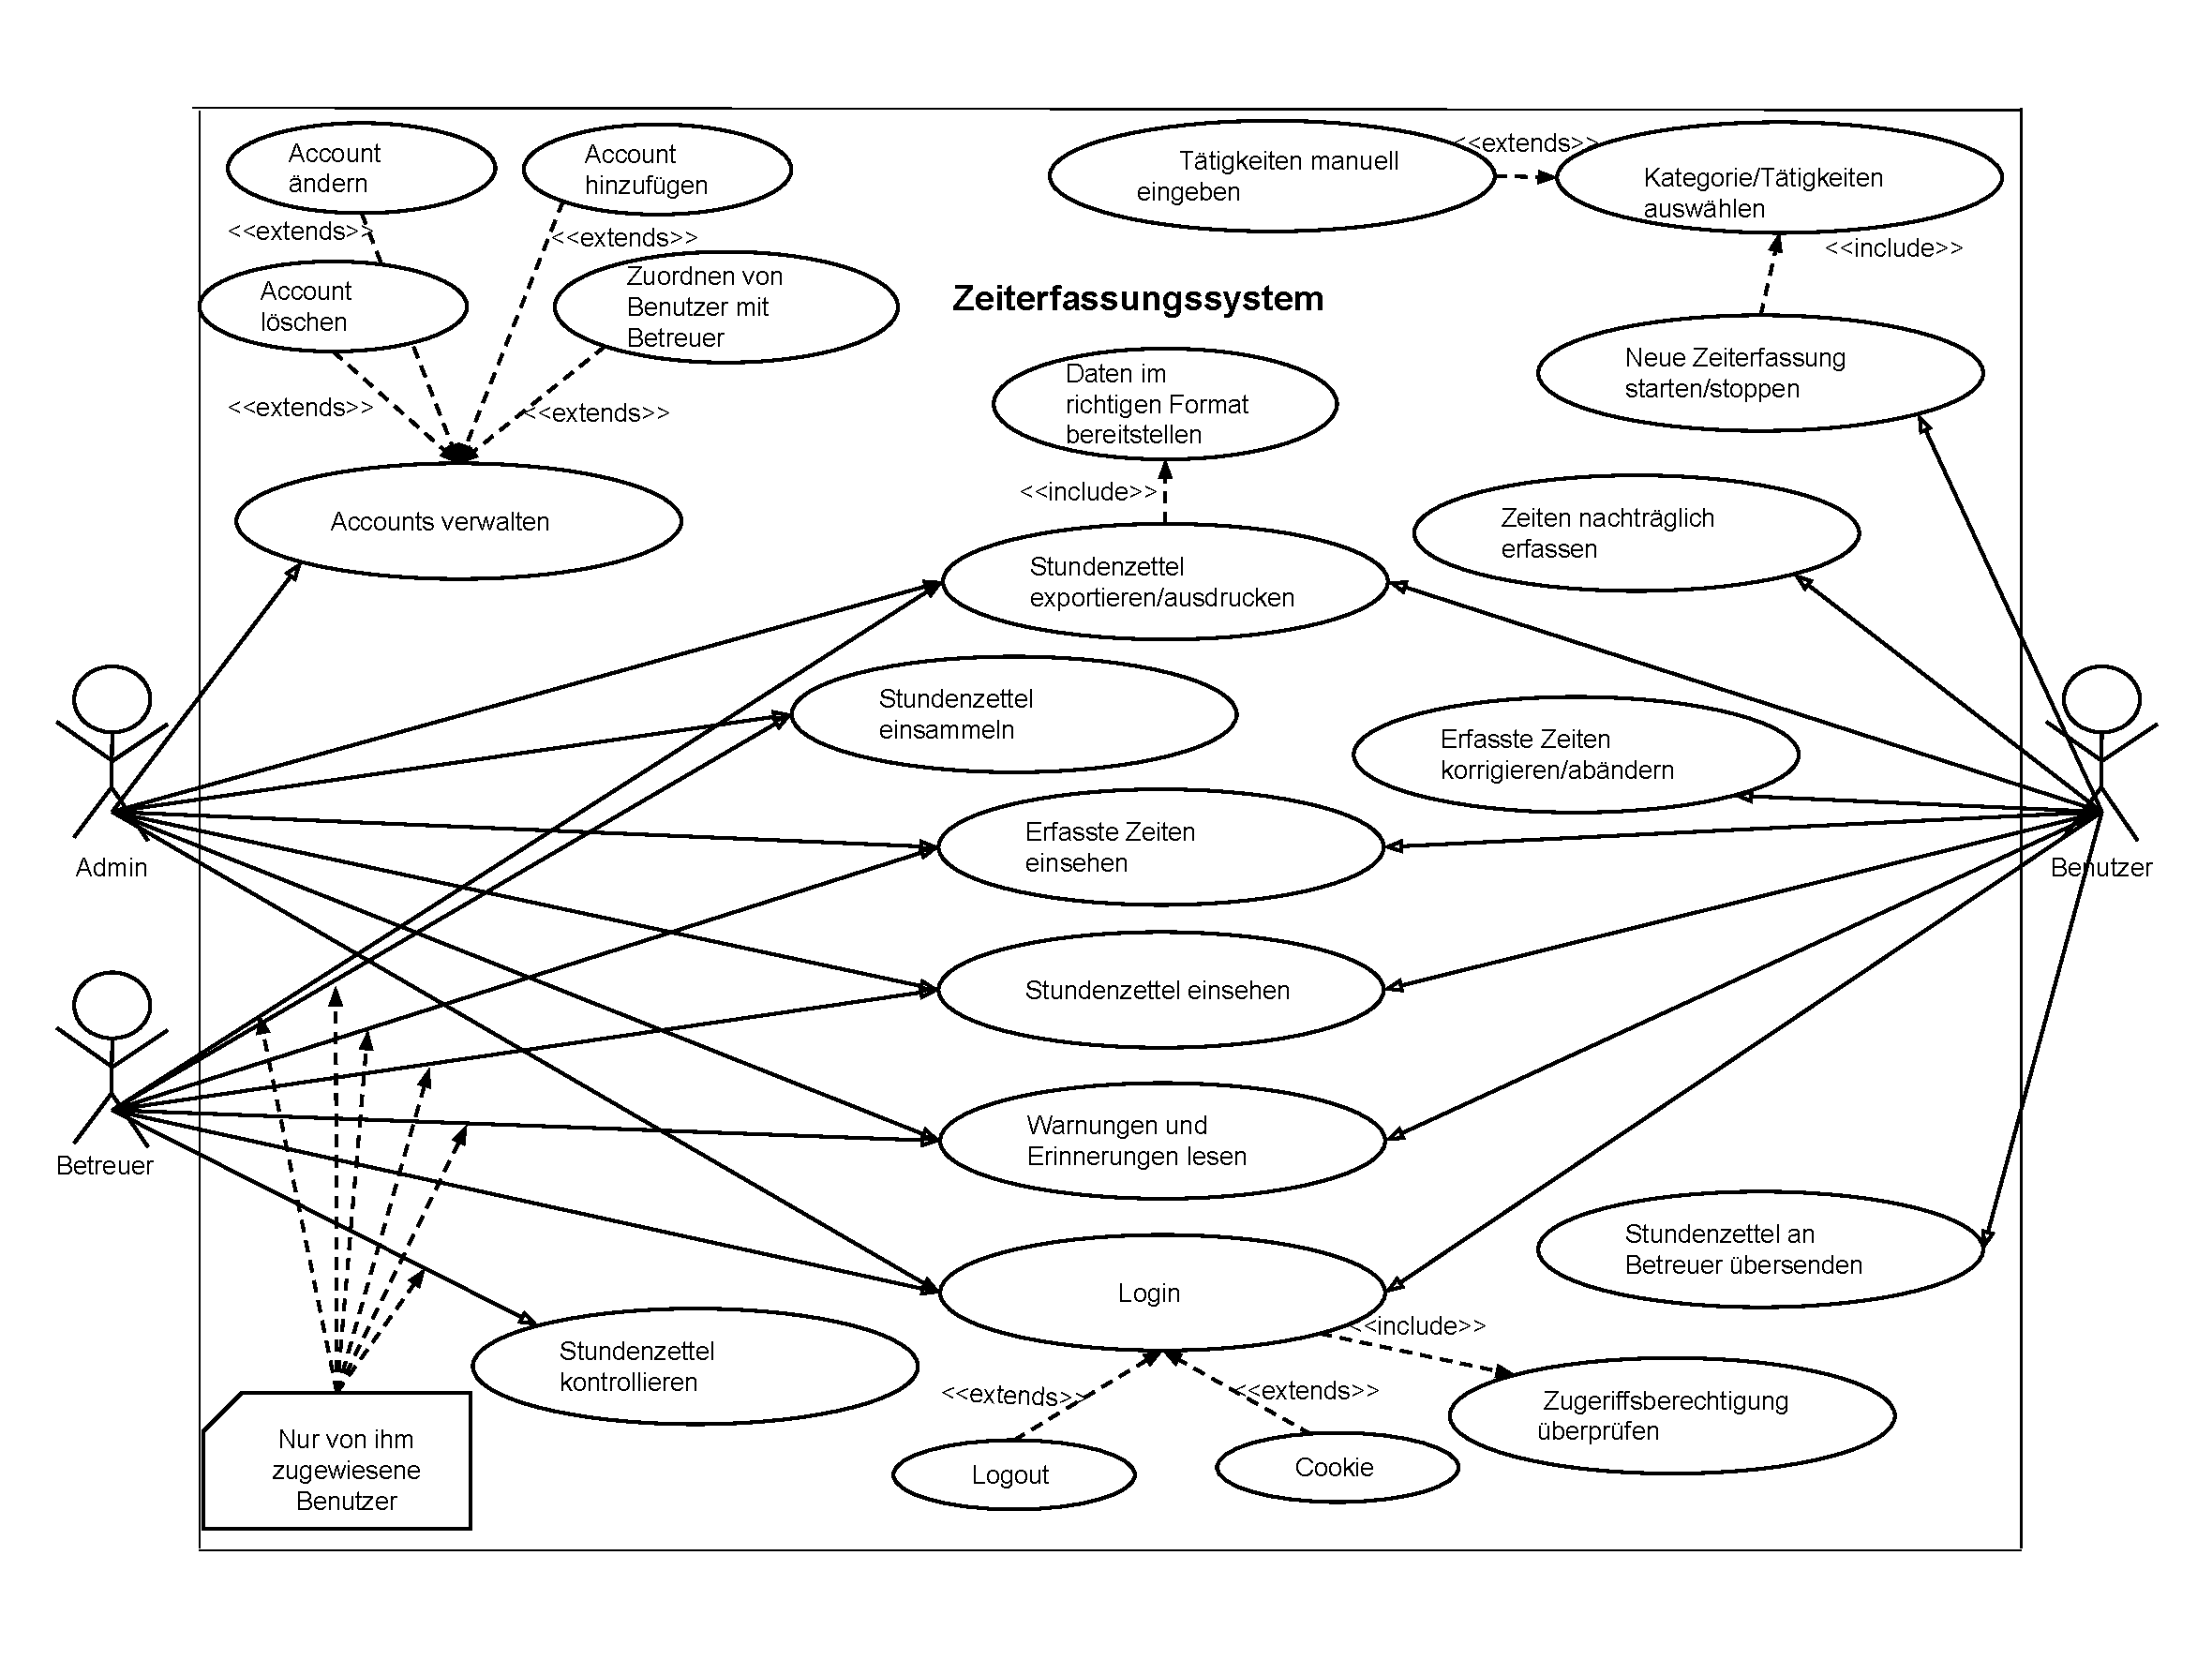
\includegraphics[width=\linewidth]{Anwendungsfalldiagramm.pdf}\\
